\section{Replacing \code{return} statements}

The \code{return} statements in the basic blocks are going to be replaced with \code{break} statements.

If the return type of the method is not \code{void}, then an assignment to the \code{ret} variable with the right-hand side
representing the expression of the \code{return} statement is added in the place of the \code{return} statement. Then the
current stack frame is popped from the stack by a call to \code{pop()} on the \code{stack} object. Finally, a
\code{break} statement is added to the parent block of the \code{return} statement. The target of this \code{break}
statement needs to be the \code{switch} statement enclosing the basic blocks. This is why if there is at least one
\code{return} statement in the method which is still included in a loop after generating the basic blocks, the
\code{switch} statement enclosing the basic blocks will get a \code{label} called \code{switchLabel}. The \code{break}
statements corresponding to \code{return} statements still enclosed in loops after generating the basic blocks will also
have the label \code{switchLabel}. Otherwise, these \code{break} statements would transfer control to the statement after
the enclosing loop and not to the statement after the \code{switch} statement, as it should happen.

An example of this pass is provided in \labelindexref{Figure}{img:return}.

\begin{figure}[htb]
    \makebox[\linewidth][c]{%
    \begin{subfigure}[b]{.6\textwidth}
        \centering
        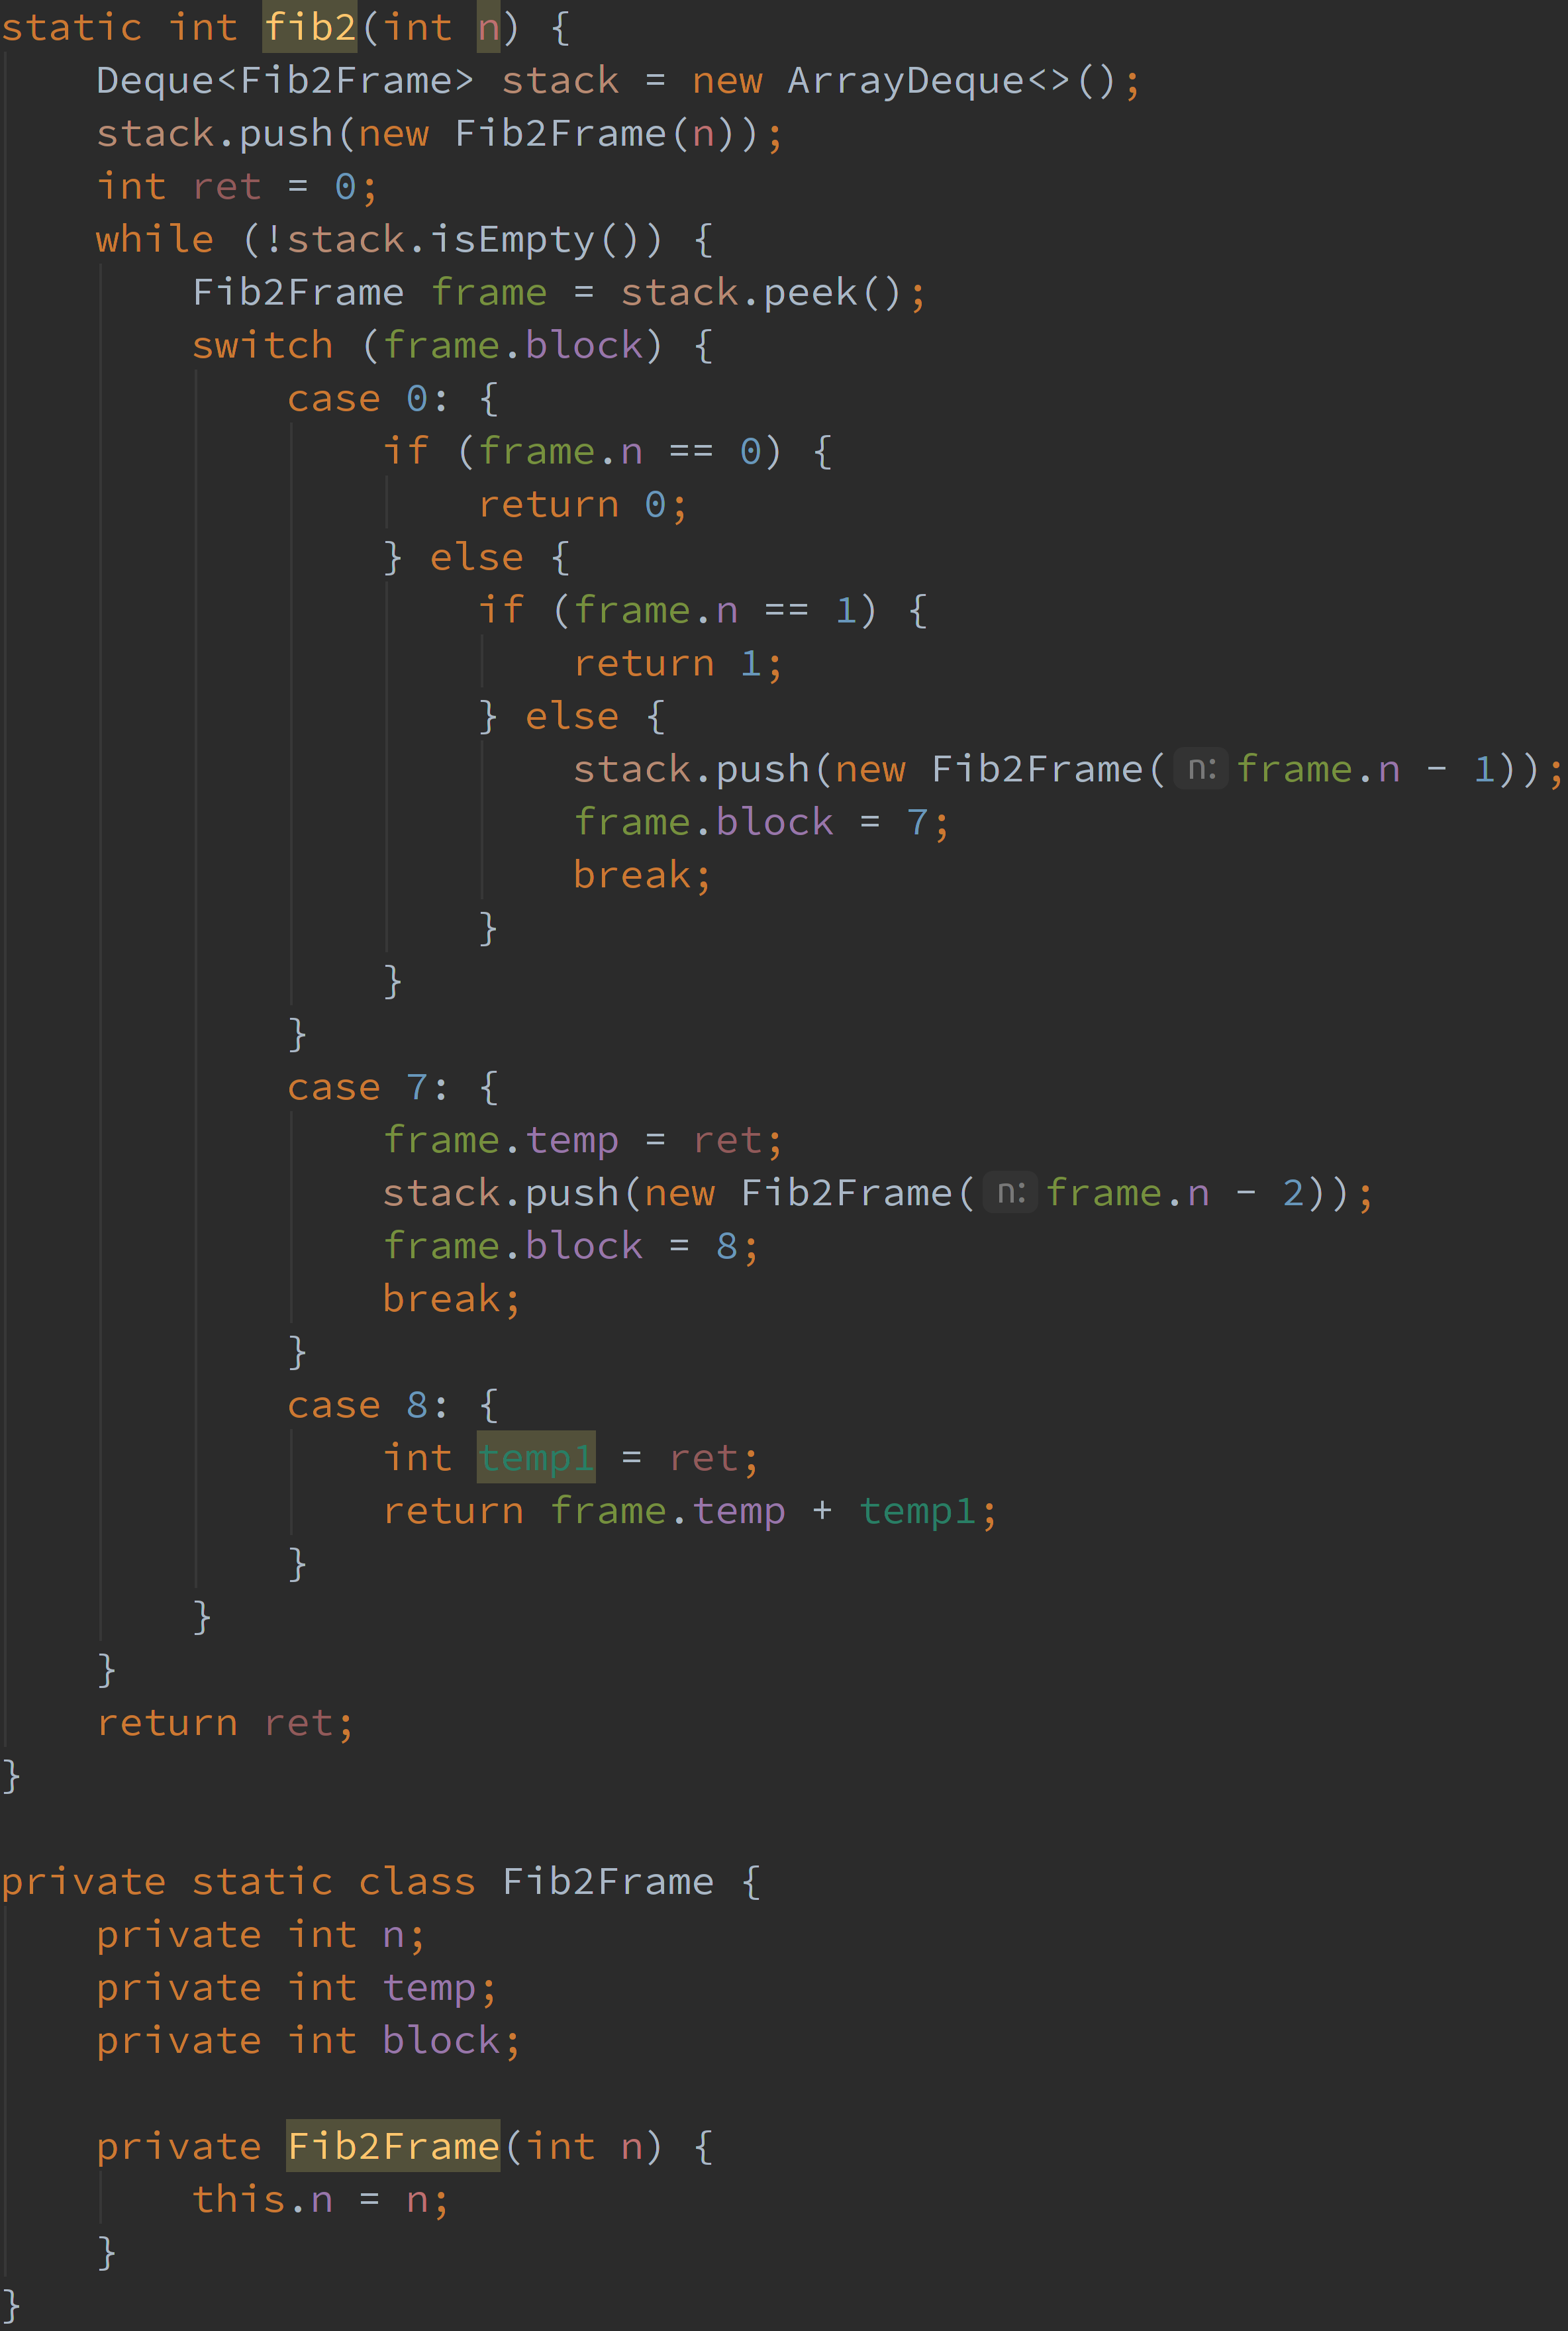
\includegraphics[height=5in]{src/img/inline-blocks-after-44.png}
        \caption{Before}
    \end{subfigure}%
    \begin{subfigure}[b]{.6\textwidth}
        \centering
        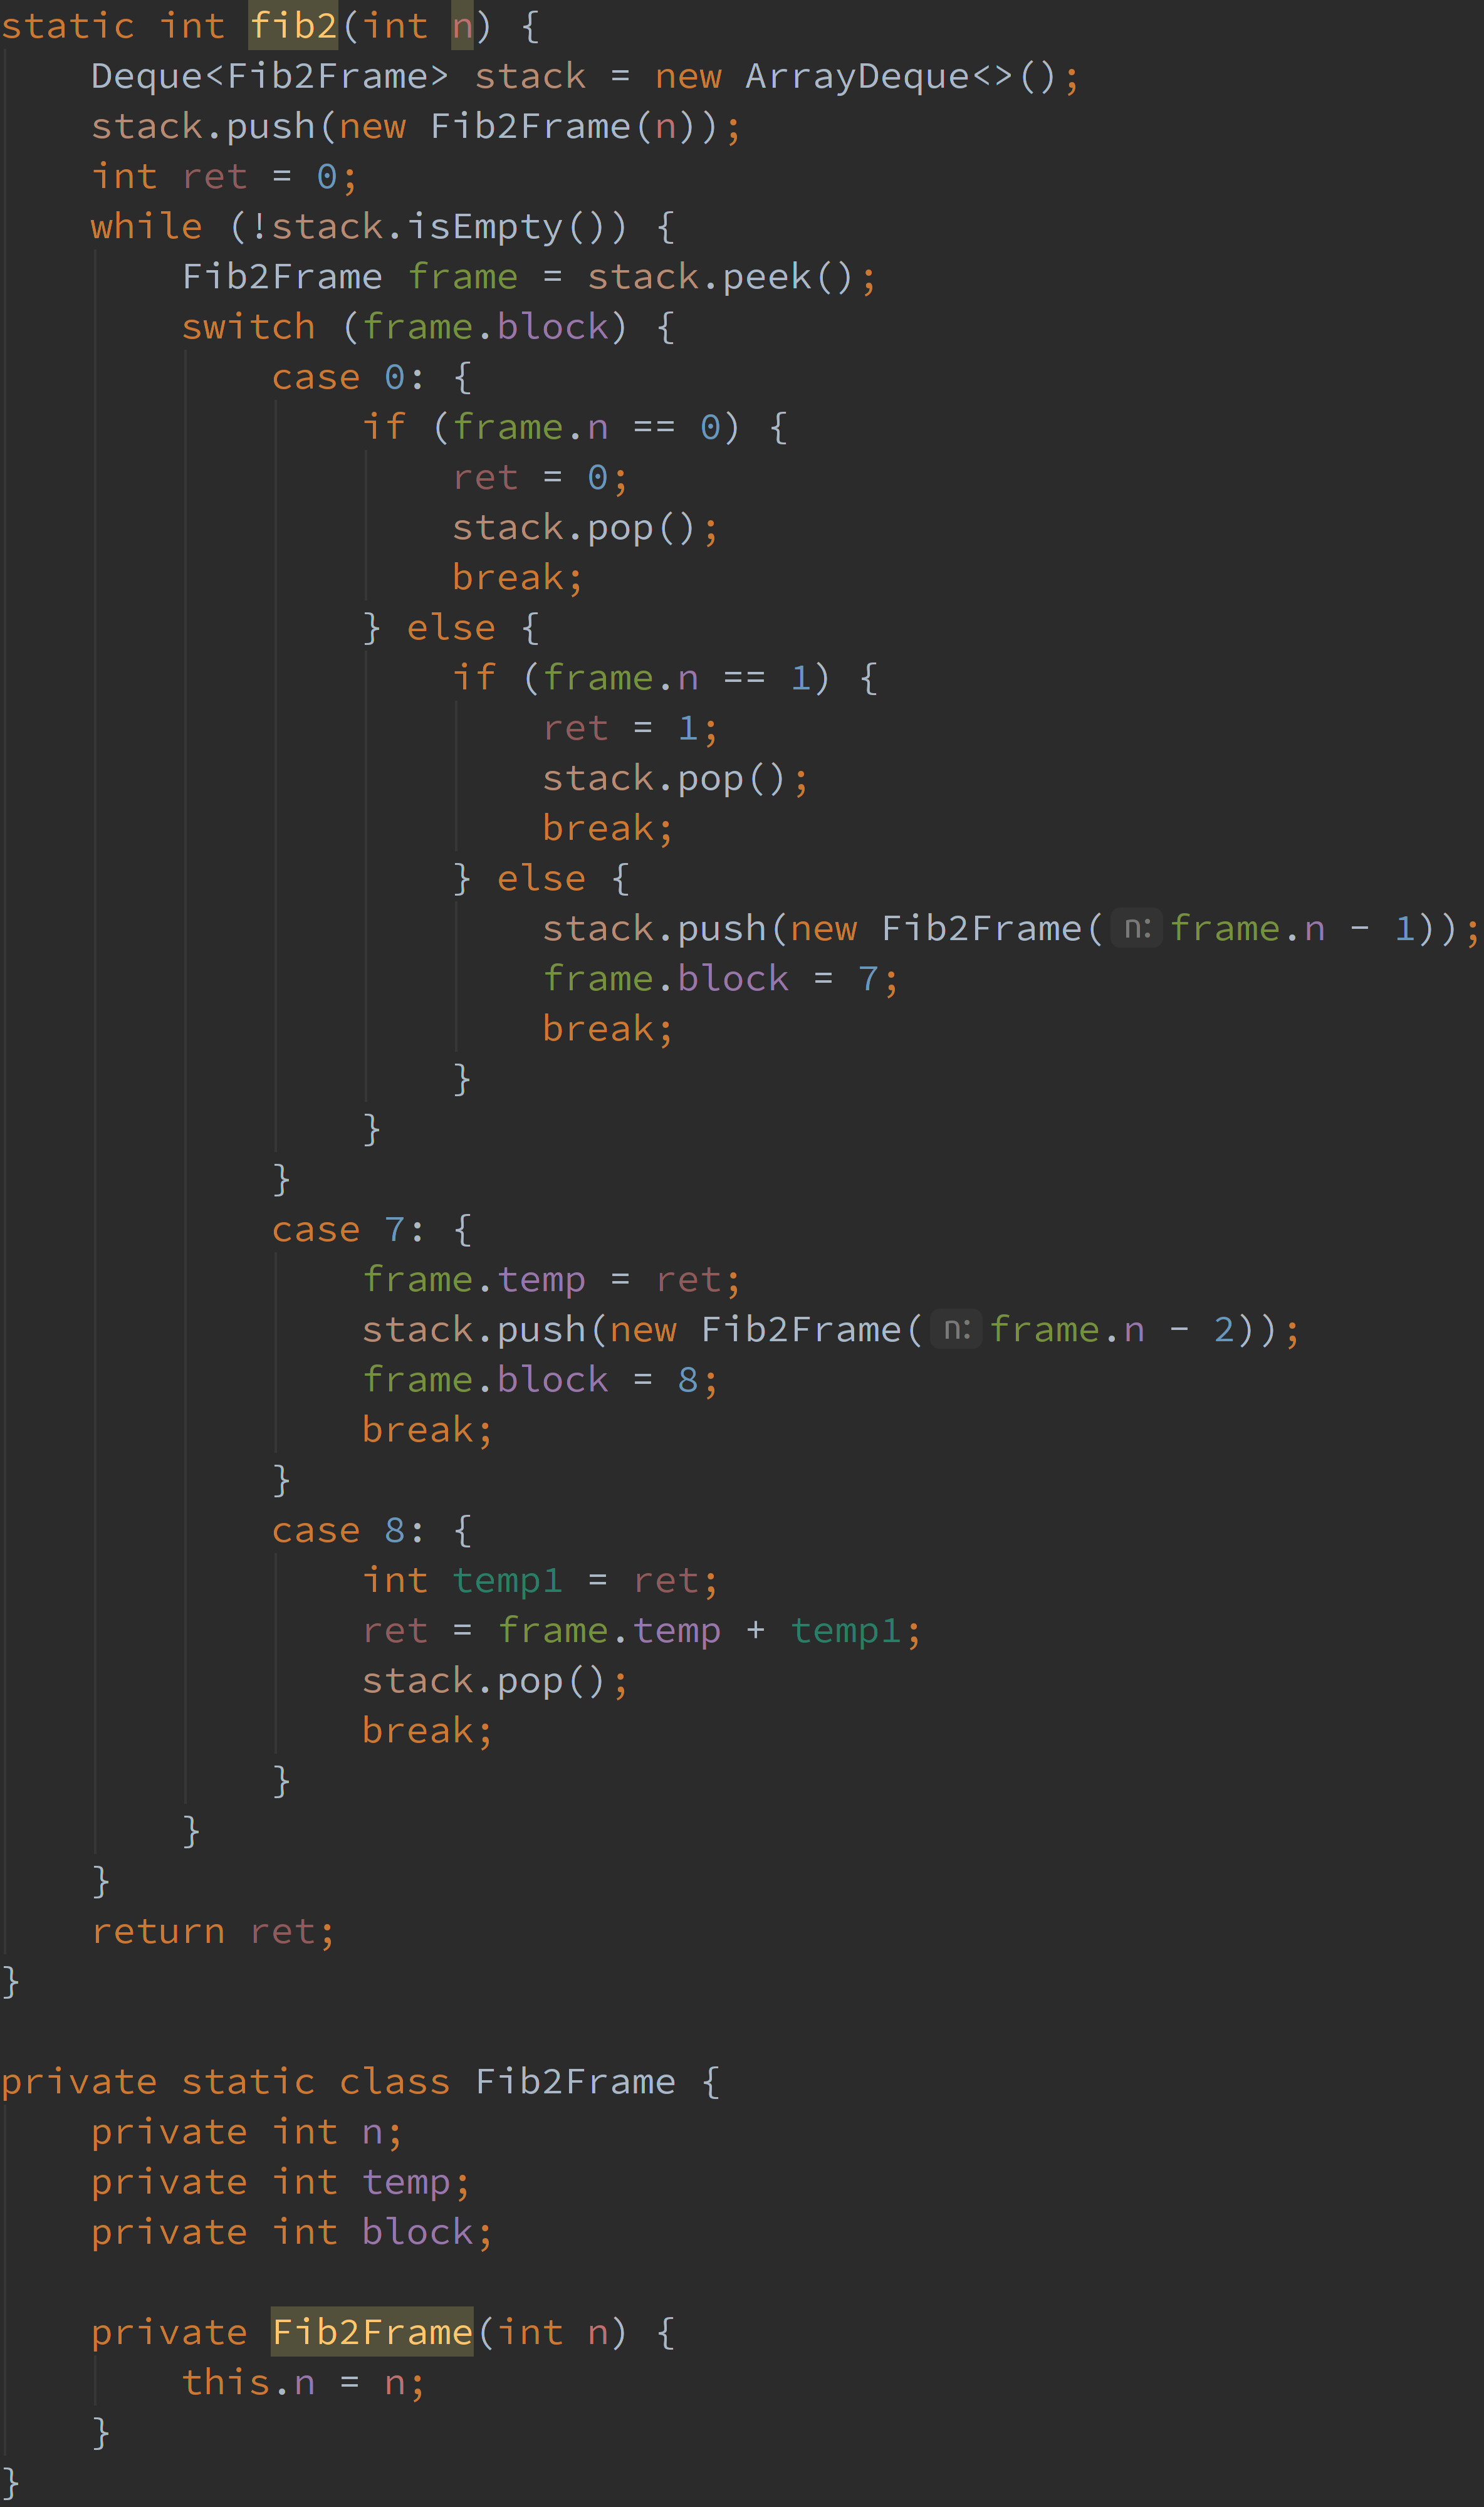
\includegraphics[height=5.682in]{src/img/return-after.png}
        \caption{After}
    \end{subfigure}%
    }\\
    \caption{Replacing \code{return} statements \label{img:return}}
\end{figure}